\documentclass[tikz,border=2pt]{standalone}
\usepackage{amsmath,amssymb}
\usepackage{pgfplots}
\pgfplotsset{compat=1.18}

\begin{document}
% A polynomial on R^2 is a finite sum of monomials; here the degree-3 polynomial
% p(x1,x2) = x1^3 - 3 x1 x2^2 (the "monkey saddle").
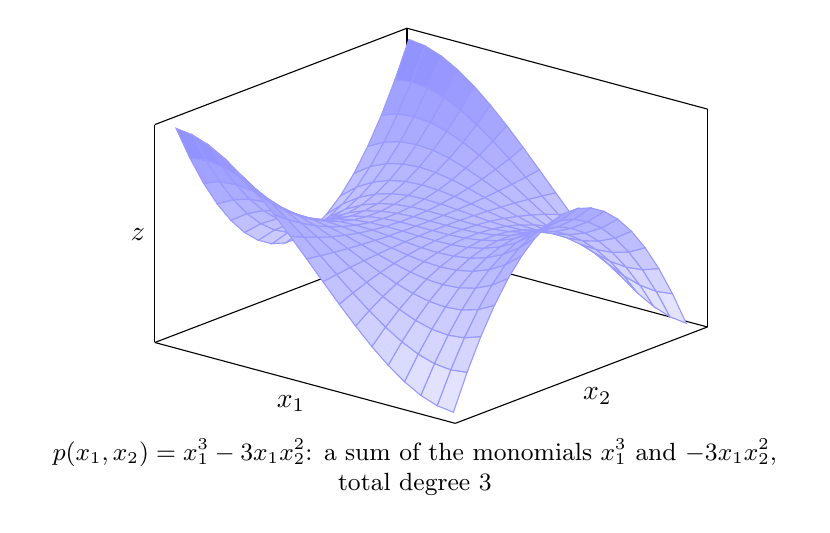
\begin{tikzpicture}
	\begin{axis}[
		view={40}{30},
		xmin=-1.3, xmax=1.3, ymin=-1.3, ymax=1.3, zmin=-3.6, zmax=3.6,
		xlabel={$x_1$}, ylabel={$x_2$}, zlabel={$z$},
		zlabel style={rotate=-90},
		xtick=\empty, ytick=\empty, ztick=\empty,
		width=8.6cm, height=6.6cm
		]
		\addplot3[surf, shader=faceted, faceted color=blue!40, colormap={pale}{color=(blue!8) color=(blue!45)}, samples=18, domain=-1.2:1.2, domain y=-1.2:1.2, z buffer=sort] {x^3-3*x*y^2};
	\end{axis}
	\node[anchor=north, align=flush center, text width=9.6cm, font=\small] at ([yshift=-2pt]current axis.outer south) {$p(x_1,x_2)=x_1^3-3x_1x_2^2$: a sum of the monomials $x_1^3$ and $-3x_1x_2^2$, total degree $3$};
\end{tikzpicture}
\end{document}
